\documentclass[12pt]{article}

\usepackage{mathrsfs}
\usepackage{epsfig}
\usepackage{graphicx}
\usepackage{color}
\usepackage{amsmath}
\usepackage{amsfonts}
\usepackage{amssymb}
\usepackage{amsthm}
\usepackage{amscd}
\usepackage{verbatim}
\usepackage{fullpage}
\usepackage{indentfirst}

%\setcounter{MaxMatrixCols}{20}
\theoremstyle{plain}
\newtheorem{theorem}{Theorem}[section]
\newtheorem{proposition}[theorem]{Proposition}
\newtheorem{lemma}[theorem]{Lemma}
\newtheorem{corollary}[theorem]{Corollary}
\newtheorem{conjecture}[theorem]{Conjecture}
\theoremstyle{definition}
\newtheorem{definition}[theorem]{Definition}
\newtheorem{notation}[theorem]{Notation}
\newtheorem{remark}[theorem]{Remark}
\newtheorem{example}[theorem]{Example}
\numberwithin{equation}{theorem}

\newcommand{\black}{\hfill{\ensuremath{\blacksquare}}}
\DeclareMathAlphabet{\mathpzc}{OT1}{pzc}{m}{it}

\graphicspath{ {./} }

\begin{document}
\begin{titlepage}
	\centering
	\vspace{4cm}
	{\scshape\Large DSE 220: Machine Learning\par}
	\vspace{1.5cm}
	{\huge\bfseries Homework 4: Embedding of Words\par}
	\vspace{2cm}
	{\Large\itshape Kevin Kannappan\par}

% Bottom of the page
	{\large \today\par}
\end{titlepage}


\section{100-Dimensional Embedding Description}

The Brown Corpus was developed in the 1960s and it contains 500 samples of English language text, totaling roughly 1 million words (Wikipedia). Leveraging the documentation found in the assignment, we found that the initial document found on NLTK contains $\approx$ 1.16M separate elements which were filtered down to remove both punctuation and ''stop" words (or words considered to be useless based on high frequency and no informative value). Hence, we were left with $\approx$ 54K unique and valuable words to be leveraged for our embedding.

\bigskip
Utilizing a counter function, we were able to aggregate the counts of the occurrence of each word and sort them in order from most frequent to least. From that sorted list, we generated a \textit{vocabulary} \textbf{V} and \textit{context words} \textbf{C} based on the first 5000 and 1000 words respectively. Using those two lists, we were able define a probability distribution based on the number of context words, $c \in C$, surrounding the words in our vocabulary, $w \in V$, as $Pr(c|w)$. We also defined an overall distribution of the context words $Pr(C)$, both of which are distributions over \textbf{C}.

\bigskip
The last prerequisite step prior to building our 100-dimensional embedding was to generate the positive point-wise mutual information matrix, where effectively each word in the vocabulary has a C-dimensional vector indicating the likelihood of context words appearing with that vocabulary. This is defined as $\phi (w) = max(0,\log \frac{Pr(c|w}{Pr(C)})$ where the log scale is leveraged to reduce skew. At this point, our data is 1000-dimensional with relevant contextual information on relevant words around the target vocabulary words. To create our 100-dimensional embedding, $\psi(w) \in R^{100}$, we apply \textbf{Principal Component Analysis (PCA)} to reduce the dimensionality of our context words to our top 100 eigenvectors representative of the variance of those words. PCA was chosen since it has been proven robust for linear dimensional embedding, an assumption that was validated by subsequent results (outlined in Sections 2 and 3). The result of the PCA transformation removed a substantial amount of the variance, leaving $\approx$ 23\% explained in the resulting embedding (depicted below):
\bigskip

\begin{center}
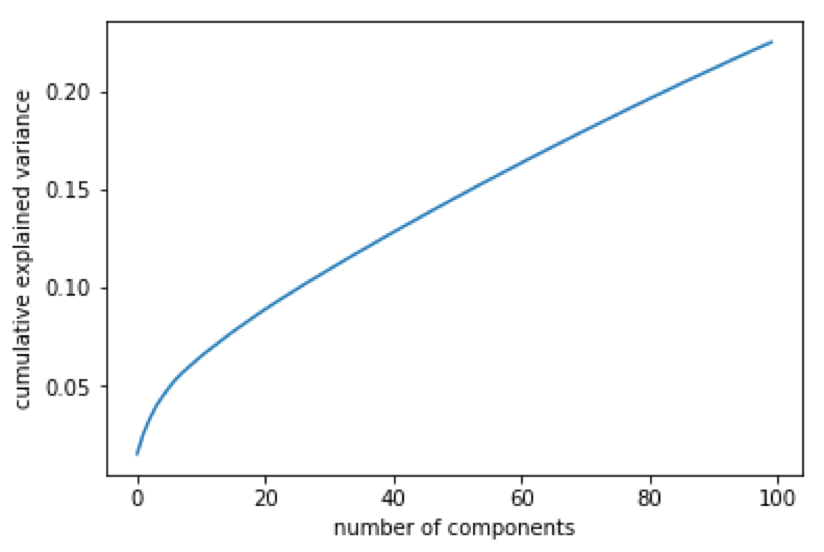
\includegraphics[width=8cm, height=6cm]{pca_100}
\end{center}
\bigskip
\bigskip

\section{Nearest Neighbor Results}
\subsection{Method and Description}

A subset collection of words was selected from the embedding and \textbf{K Nearest Neighbors (with K=1)} was applied to return its nearest neighbor. Using cosine distance as given was proven to be quite effective, as the following results were intuitive. The most naive neighbor search implementation involves the ''brute-force" computation of distances between all pairs of points in the dataset, which was implemented since the data no longer had large dimension constraints.

\subsection{Results and Analysis}

Nearest Neighbor results of the selected words are depicted in the figure below:
\bigskip

\begin{center}
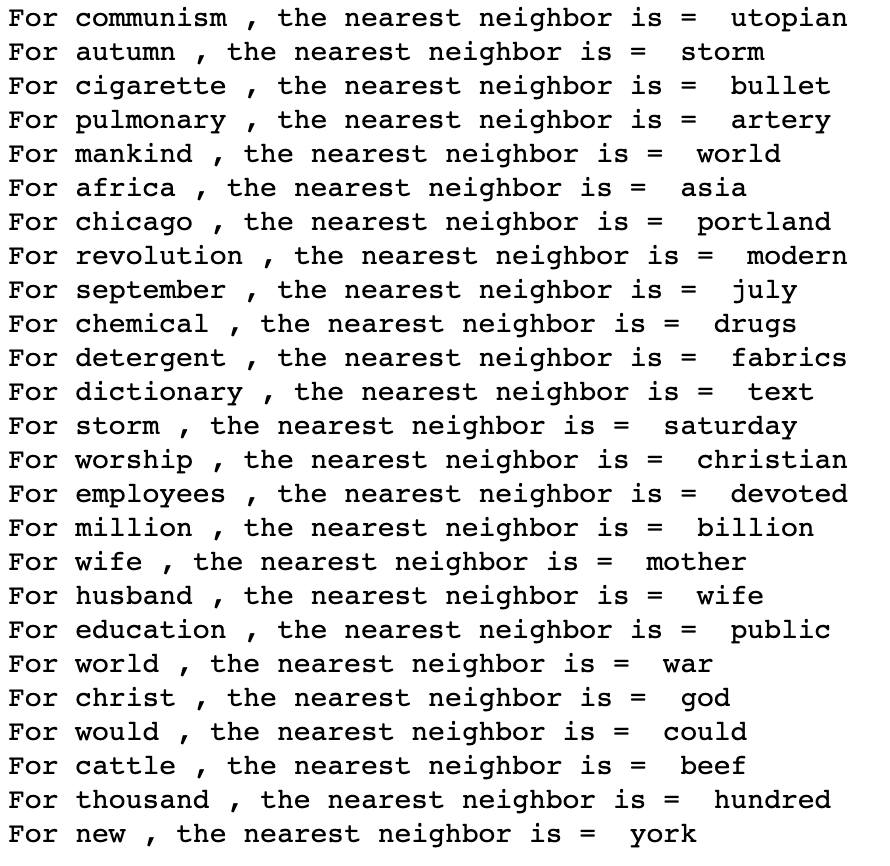
\includegraphics[width=10cm, height=10cm]{nn_100}
\end{center}
\bigskip

\bigskip
In the sample of 25 words, only 2 appear to be counterintuitive: cigarrette matched with bullet and storm matched with saturday. Otherwise, the resulting values appear to be doing very well with both outlier words (communism to utopian) and common words (would to could). In conclusion, the nearest neighbor algorithm was successful in finding relevant related words. Future research could experiment with different distance metrics or higher values of K to see the collections of nearby words. There would be little value to tuning the search implementation as the data-size is still small.


\section{Clustering}
\subsection{Method and Description}

Using the vectorial representation of the embedding, we clustered the data into 100 separate clusters using the \textbf{K-Means++} algorithm. The advantage of K-Means++ is that its centroid selection is not random and it is better able to approximate the true center than regular K-Means as there are likely outlier values present. The algorithm used was the default method since our data is dense and did not need to be tuned. Lastly, the value of the number of times that the algorithm would be run with different centroid seeds (n init) was tuned so as to minimalize redudancy with higher n init values.

\subsection{Results and Analysis}

Sample (best) K-Means clusters are depicted in the figure below:
\bigskip

\begin{center}
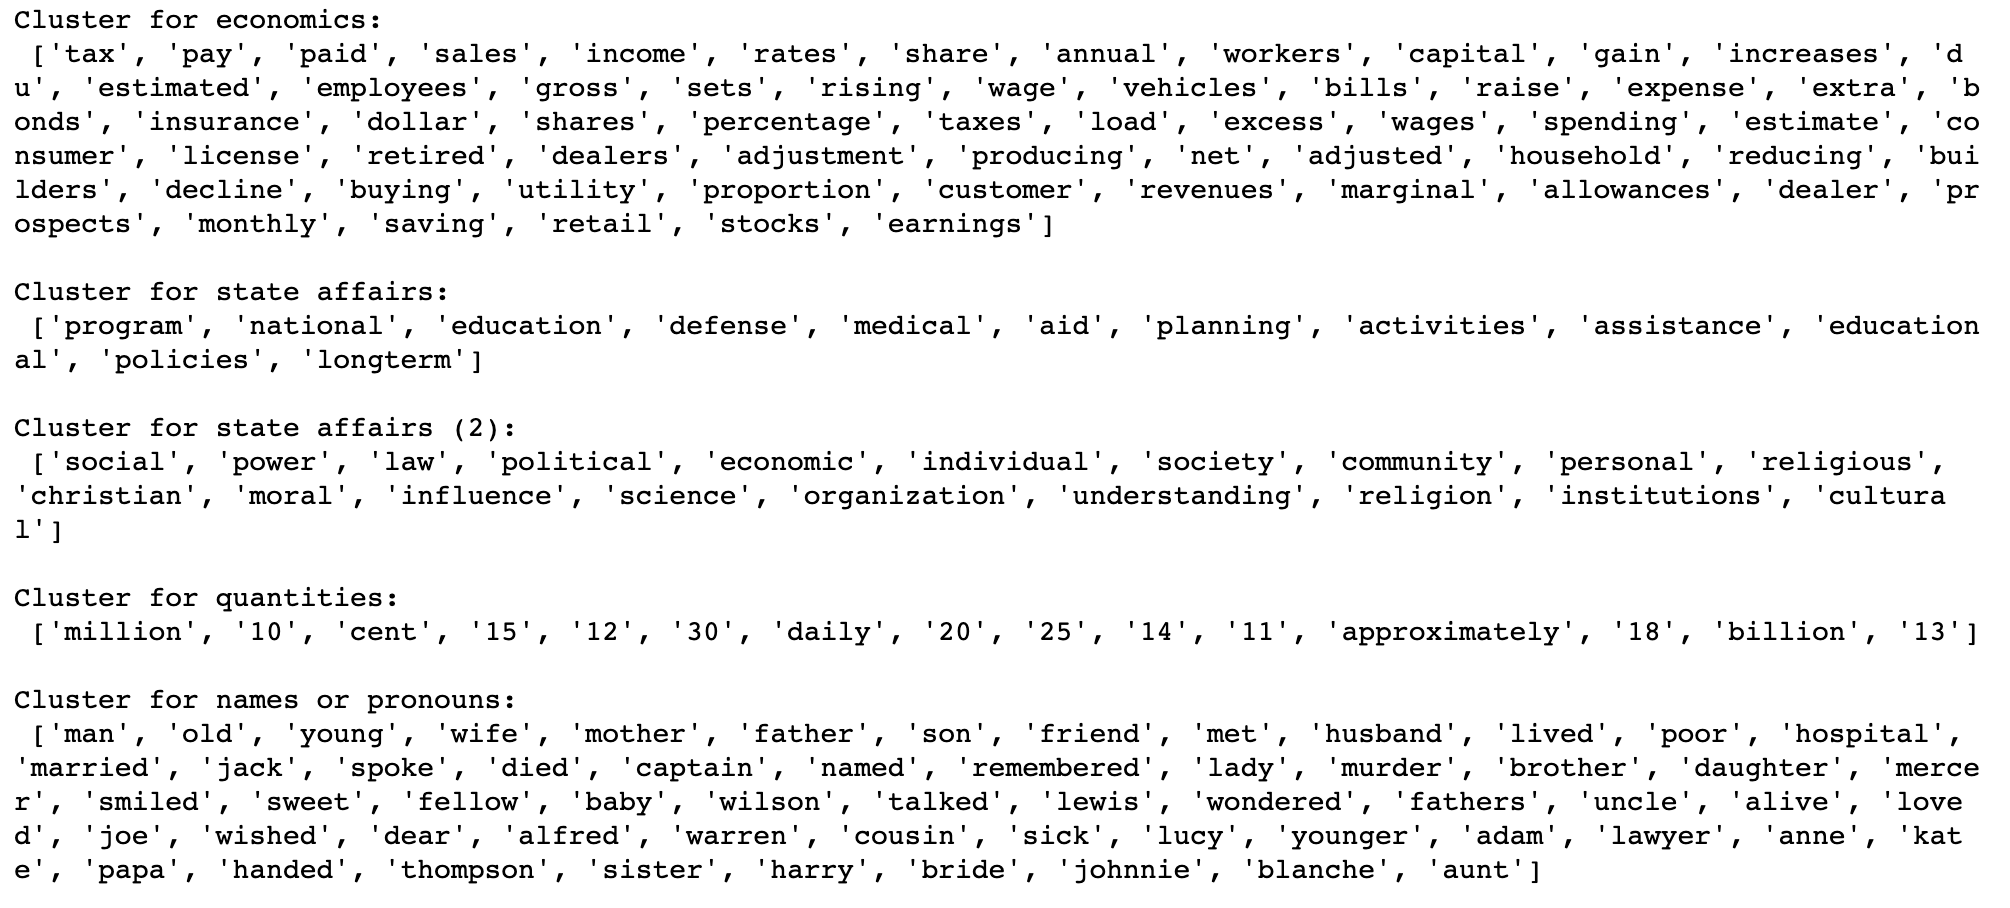
\includegraphics[width=16cm, height=10cm]{kmeans_100}
\end{center}
\bigskip

\bigskip
The clusters definitely appear to be moderately coherent. Values (numbers), subjects (names and pronouns), and even more granular clusters like economics or political areas are clustered together as well. Future research would benefit with less clusters, as some of the words appear to be clustered in smaller subsets than intuitively would make sense. Hence, larger groups of words would be able to provide more insight - potentially leaving space to investigate \textbf{Hierarchical Clustering}. In terms of the tuned algorithm implemented, I am not sure changing the other hyperparameters would provide a performance (more coherence) increase.


\section{Conclusion}

Based on analyses of performance in clustering and nearest neighbor approaches, we can safely conclude that the 100-dimensional embedding chosen is an effective one. Improvements in both areas were highlighted in the corresponding sections. With regards to improving the utility of the embedding data, there are possibilities to use non-linear dimensionality reductions (e.g. Isomap), yet considering the effectiveness of PCA, they were not pursued. There are shortcomings with producing the embedding, as the loop written was very inefficient - potentially parallelism would help to reduce the computational requirements. Above all, the code and decisions made were to optimize over the Brown Corpus.

\end{document}